\subsection{简约波矢$\vec k$的取值和物理意义}
为了确定波矢$\vec k$的值,必须引入边界条件。选择周期性边条件(也称Born-Von Karman条件)。
\begin{equation}
  \left\{
  \begin{aligned}
     \psi(\vec r+N_1\vec{\mathbf a}_1)&=\psi(\vec r)\\
     \psi(\vec r+N_2\vec{\mathbf a}_2)&=\psi(\vec r)\\
     \psi(\vec r+N_3\vec{\mathbf a}_3)&=\psi(\vec r)\\
   \end{aligned}\right.
  \label{eq:solid-31}
\end{equation}
其中$\vec{\mathbf a}_i(i=1,2,3)$是Bravais格子的三个基矢,$N_1$、$N_2$、$N_3$分别是沿着基矢$\vec{\mathbf a}_1$、$\vec{\mathbf a}_2$、$\vec{\mathbf a}_3$方向的原胞数,$N=N_1N_2N_3$是晶体中的原胞总数。因此$\vec k$(相应的本征值$\lambda_{\vec R_n}$)的取值将受到限制。根据Bloch定理,%将式\eqref{eq:bloch}代入\eqref{eq:solid-31}得
\begin{equation}
  \psi(\vec r+N_i\vec{\mathbf a}_i)=e^{iN_i\vec k\cdot\vec{\mathbf a}_i}\psi(\vec r),\quad i=1,2,3
  \label{eq:solid-32}
\end{equation}
这就要求$e^{iN_i\vec k\cdot\vec{\mathbf a}_i}=1$,
%\begin{equation}
%  e^{iN_i\vec k\cdot\vec{\mathbf a}_i}=1,\quad i=1,2,3
%  \label{eq:solid-33}
%\end{equation}
%或者等价地
%\begin{equation}
%  N_i\vec k\cdot\vec{\mathbf a}_i=2\pi l_i,\quad l_i\mbox{为整数},\quad i=1,2,3
%  \label{eq:solid-34}
%\end{equation}
将波矢$\vec k$用相应的倒格子的基矢$\vec{\mathbf b}_i(i=1,2,3)$表示,%即
%\begin{equation}
%  \vec k=k_1\vec{\mathbf b}_1+k_2\vec{\mathbf b}_2+k_3\vec{\mathbf b}_3
%  \label{eq:solid-35}
%\end{equation}
%代入式\eqref{eq:solid-34},并
利用正交关系式\eqref{eq:solid-12}$\vec{\mathbf a}_i\cdot\vec{\mathbf b}_j=2\pi\delta_{ij}$,%有
%\begin{equation}
%  \vec k=\dfrac{l_1}{N_1}\vec{\mathbf b}_1+\dfrac{l_2}{N_2}\vec{\mathbf b}_2+\dfrac{l_3}{N_3}\vec{\mathbf b}_3
%  \label{eq:solid-36}
%\end{equation}
许可的简约波矢$\vec k$可以看成是倒格子空间中以$\dfrac{\vec{\mathbf b}_i}{N_i}(i=1,2,3)$为基矢的Bravais格子的格矢。


每个许可的$\vec k$值由上述Bravais格子的格点表示,在$\vec k$空间内所占的体积
\begin{equation}
  \Delta\vec k=\dfrac{\vec{\mathbf b}_1}{N_1}\cdot\biggl(\dfrac{\vec{\mathbf b}_2}{N_2}\times\dfrac{\vec{\mathbf b}_3}{N_3}\biggr)=\dfrac1N\vec{\mathbf b}_1\cdot(\vec{\mathbf b}_2\times\vec{\mathbf b}_3)
  \label{eq:solid-37}
\end{equation}
由于$\vec{\mathbf b}_1\cdot(\vec{\mathbf b}_2\times\vec{\mathbf b}_3)$是倒格子原胞的体积,因此倒格子空间原胞许可的$\vec k$的数目等于实空间中晶体的总的原胞数目。


倒格子原胞体积为$\dfrac{(2\pi)^3}{\Omega_0}$,%式\eqref{eq:solid-14},
$\Omega_0$是正格子的原胞体积,$N\Omega_0=V$,因此$\vec k$空间中许可态的态密度
\begin{equation}
  \dfrac1{\Delta\vec k}=\dfrac V{8\pi^3}
  \label{eq:solid-38}
\end{equation}
对于用平面波描述的自由电子,$\hbar\vec k$是电子的动量\cite{Yanshousheng}。但是对于Bloch电子,简约波矢$\vec k$并不比例于电子的动量。动量算符$p=-i\hbar\nabla$作用于Bloch波函数%(式\eqref{eq:blochpw})上,
\begin{equation}
  \begin{split}
  -i\hbar\nabla\psi_{\vec k}&=-i\hbar\nabla(e^{i\vec k\cdot\vec r}u_{\vec k}(\vec r))\\
  &=\hbar\vec k\psi_{\vec k}-i\hbar e^{i\vec k\cdot\vec r}\nabla u_{\vec k}(\vec r)
  \end{split}
  \label{eq:solid-39}
\end{equation}
并不能写成一个简单的常数乘以$\psi_{\vec k}$,因此$\psi_{\vec k}$也不是动量算符的本征函数。


简约波矢$\vec k$是对应于平移操作本征值的量子数,它的物理意义是表示原胞之间电子波函数位相的变化。不同$\vec k$值表明原胞间的位相是不同的。但是需要指出的是,如果$\vec k$改变一个倒格子矢量
\begin{displaymath}
  \vec G_n=n_1\vec{\mathbf b}_1+n_2\vec{\mathbf b}_2+n_3\vec{\mathbf b}_3,\quad(n_1,n_2,n_3\mbox{为整数})
\end{displaymath}
完全不会影响本征值$\lambda_{\vec R_n}$。因此,为了使$\vec k$能与平移算符的本征值$\lambda_{\vec R_n}$一一对应,必须要把$\vec k$的取值限制在一定的范围之内,使得它既能概括所有不同的本征值$\lambda_{\vec R_n}$的取值,同时又没有任意两个$\vec k$相差一个倒格矢$\vec G_n$。最方便的办法是将$\vec k$限制在$\vec k$空间的WS原胞中。

\subsection{$\vec k$-空间中积分}
利用平移对称性,晶体的物理性质的计算可以表示为第一Brillouin区的积分。实际计算的时候,取$\vec k$-空间中用有限格点的Hamiltonian的本征值和本征矢进行计算。为使Brillouin区积分达到要求的精度,一般需要计算$\vec k$-空间中$10^3\sim10^4$个格点的本征值$E(\vec k)$和本征矢$\Psi(\vec k)$。这种直接积分布点计算的方法计算晶体能带结构非常笨拙,很难应用于需要大量$\vec k$点的体系,因此必须采用插值方法。

插值方法可以分为数学和物理插值两类,后者包括赝势经验方法\cite{SSP18-165_1966},$\widehat{\vec k\cdot\vec p}$方法\cite{Kane,JCP6-367_1938,Seitz,xie-lu};紧束缚近似的Slater-Koster公式和模型Hamiltonians方法\cite{Nemoshkalenko-Aleshin}。实际计算中,经常使用的是数学插值,包括线性插值\cite{PR144-390_1966,PSSB54-469_1972}和二次插值\cite{PRA139-489_1965,PLA28-570_1969,AP67-15_1971}。

\subsubsection{四面体线性插值和二次插值}\label{Tetrahedron-Quadratic}
线性插值是Gilat和Raubenheimer\cite{PR144-390_1966}为计算声子态密度而提出的。

晶体中电子态密度的线性插值计算公式为:
\begin{equation}
  N(E)=\frac1N\sum_{\vec k}\delta(E-E(\vec k))=\frac1{\Omega_0}\int d^3\vec k\delta(E-E(\vec k)) 
  \label{eq:solid-193}
\end{equation}
Brillouin区被分为小的正方体,在每个正方体中$E(\vec k)$,能量在立方体中心波矢$\vec k_0$附近展开到包含一阶导数,
\begin{equation}
  E(\vec k)=E(\vec k_0)+(\vec k-\vec k_0)\nabla E(\vec k)|_{\vec k=\vec k_0}
  \label{eq:solid-194}
\end{equation}
态密度表达式\eqref{eq:solid-193}可以变换为对常数能量的表面积分
\begin{equation}
  N(E)=\frac2{(2\pi)^3}\int_S\frac{dS}{|\nabla_{\vec k}E(\vec k)|_{\vec k-\vec k_0}}
  \label{eq:solid-195}
\end{equation}
考虑到式\eqref{eq:solid-194},对Brillouin区的立方体求和代替积分,
\begin{equation}
  N(E)\simeq\frac2{(2\pi)^3}\sum_{\vec k_0}\frac{S(E,\vec k_0)}{|\nabla_{\vec k}E(\vec k)|_{\vec k=\vec k_0}}
  \label{eq:solid-196}
\end{equation}
这里$S(E,\vec k_0)$是式\eqref{eq:solid-194}所示的表面在各小立方体内的面积。通过Histogramic表示,计算这些小立方体内所含面积和对应小立方体的体心梯度可以得到晶体中的电子态密度。但是Histogramic方法应用很不方便,而且根据第一原理计算$\nabla_{\vec k}E(\vec k)$也相当麻烦。为了克服这些困难,Lehmann和Taut提出了四面体方法\cite{PSSB54-469_1972},将Brillouin区分为很多个小的四面体,计算每个四面体的四个顶点的本征态$E(\vec k)$和本征值$\Psi(\vec k)$,在四面体内部,$E(\vec k)$用线性展开的形式表示。

应用四面体方法中,积分\eqref{eq:solid-193}可以用解析表达式计算,记四面体四个顶点的能量($E_0$, $E_1$, $E_2$, $E_3$)的编号依次为$E_0\leqslant E_1\leqslant E_2\leqslant E_3$,线性插值方法中,波矢$\vec k$对应的能量$E$是一个平面(图\ref{Tetrahedron}),这里
\begin{equation}
  \begin{split}
    (1)\quad&E_0\leqslant E\leqslant E_1,\\
    (2)\quad&E_1\leqslant E\leqslant E_2,\\
    (3)\quad&E_2\leqslant E\leqslant E_3.
  \end{split}
  \label{eq:solid-197}
\end{equation}

\begin{figure}[!h]
\centering
 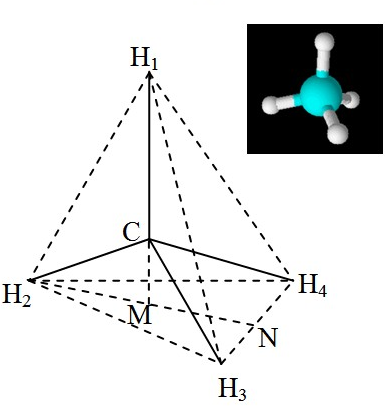
\includegraphics[width=3.35in,height=2.5in,viewport=14 14 250 190,clip]{Tetrahedron.eps}
\caption{\small Arrangement of the secant plane of constant energy in the method of tetrahedrons when $E_0\leqslant E\leqslant E_1$.}
\label{Tetrahedron}
\end{figure}

态密度的一般表达式为,
\begin{equation}
  N_A(E)=\frac1N\sum_{\vec k}A(\vec k)\delta(E-E(\vec k))=\frac{dD_A(E)}{dE}
  \label{eq:solid-198}
\end{equation}
这里
\begin{equation}
  D_A(E)=\frac1N\sum_{\vec k}A(\vec k)\theta(E-E(\vec k))
  \label{eq:solid-199}
\end{equation}
这里$\theta(x)$是Heavyside阶梯函数;$A(\vec k)$是关于矢量$\vec k$的任意函数。对应于式\eqref{eq:solid-197}的三种情况,
电子态密度的表达式分别为,
\begin{enumerate}
\item $E_0\leqslant E\leqslant E_1$
\begin{equation}
  \begin{split}
    N_A(E)=&\frac{|\vec k_{10}[\vec k_{20}\cdot\vec k_{30}]|}\Omega_0\frac{(E-E_0)^2/2}{(E_1-E_0)(E_2-E_0)(E_3-E_0)}\\
    &\cdot\left\{A_0+\left[\frac{A_1-A_0}{E_1-E_0}+\frac{A_2-A_0}{E_2-E_0}+\frac{A_3-A_0}{E_3-E_0}\right](E-E_0)/3\right\}
  \end{split}
  \label{eq:solid-200}
\end{equation}
\item $E_1\leqslant E\leqslant E_2$
\begin{equation}
  \begin{split}
    N_A(E)=&\frac{|\vec k_{10}[\vec k_{20}\cdot\vec k_{30}]|}\Omega_0\left\{\frac{(E-E_0)^2/2}{(E_1-E_0)(E_2-E_0)(E_3-E_0)}\right.\\
    &\cdot\left[A_0+\left(\frac{A_1-A_0}{E_1-E_0}+\frac{A_2-A_0}{E_2-E_0}+\frac{A_3-A_0}{E_3-E_0}\right)(E_3-E_0)/3\right]\\
    &-\frac{(E-E_1)^2/2}{(E_1-E_0)(E_2-E_1)(E_3-E_1)}\\
    &\cdot\left.\left[A_1+\left(\frac{A_1-A_0}{E_1-E_0}+\frac{A_2-A_1}{E_2-E_1}+\frac{A_3-A_1}{E_3-E_1}\right)\frac{(E-E_1)}3\right]\right\}
  \end{split}
  \label{eq:solid-201}
\end{equation}
\item $E_0\leqslant E\leqslant E_1$
\begin{equation}
  \begin{split}
    N_A(E)=&\frac{|\vec k_{10}[\vec k_{20}\cdot\vec k_{30}]|}\Omega_0\frac{(E_3-E)^2/2}{(E_3-E_0)(E_3-E_1)(E_3-E_2)}\\
    &\cdot\left\{A_3-\left[\frac{A_3-A_0}{E_3-E_0}+\frac{A_3-A_1}{E_3-E_1}+\frac{A_3-A_2}{E_3-E_2}\right](E_3-E)/3\right\}
  \end{split}
  \label{eq:solid-202}
\end{equation}
\end{enumerate}

二次插值方法选择一个大的立方体,%作为工作体积,
将该立方体分割为小的立方体,立方体的数目为$M^3$,这里$M$取决于计算要求的精度。用通过小立方体体心的三个剖面将每个小立方体分割出27个等价点,$\vec k$点的能量本征值$E(\vec k)$由27个点确定,$E(\vec k)$用小立方体内的一系列$\vec k$点展开到二阶,
\begin{equation}
  E(\vec k)=E_0+\vec m\vec k+\vec k\mathbf Q\vec k=\sum_{i=1}^{10}A_ia_i(\vec k)
  \label{eq:solid-203}
\end{equation}
这里$A_i$是展开系数;$a_i(\vec k)$是$\vec k_x$,$\vec k_y$,$\vec k_z$的线性组合到二阶。关于二次插值的详细介绍,可以参考文献\cite{AP67-15_1971}。

无论是线性插值还是二次插值,都有一些不足。对过渡金属,由于其复杂的能带结构,需要很多临界点(高对称性点)的解析结果,但是用线性插值方法则很难实现,而且态密度也主要由临界点决定,因此对临界点需要精确的解析。线性插值是对整个能带的解析积分,因此提高的是Fermi能级和Fermi面附近的态密度的计算精度。此外,线性插值方法方便处理非解析临界点(能带交叉点)的情况\cite{PLA28-570_1969,PRB7-891_1973,PRB5-1276_1972}。

能带交叉是积分误差的主要来源,在Brillouin区中接近交叉点的小区域内$|\nabla_{\vec k}E(\vec k)|\simeq0$,形成$N(E)$的能量奇点,导致不正确的插值计算,伴随能带交叉产生的另外一个问题是交叉点附近不同可观测物理量的矩阵元的行为。能带交叉导致矩阵元在交叉点变化剧烈,如果插值点位于这些交叉点上,可能引起更大的误差。理论上,计算精度可以通过增加线性插值的四面体数目或者二次插值中的参数$M$来提高,因此计算精度主要由布点数目决定。

四面体线性插值和二次插值是晶体计算中使用最多的积分方法。有时常将两种方法结合使用,用二次插值计算各参考点的线性插值部分,然后用线性四面体方法计算积分。与之类似的思想就是混合插值,用二次插值得到式\eqref{eq:solid-194}中的梯度
\begin{equation}
  \nabla E(\vec k)=\sum_{i=1}^{10}A_i\nabla C_i(\vec k)
  \label{eq:solid-204}
\end{equation}
这里$C_i(\vec k)$式$k_x$,$k_y$,$k_z$的简单解析函数。

\subsubsection{特殊点方法}
特殊点方法积分中用位于高对称性位置的$\vec k$点附近,以该特殊点作代表,用权重求和代替积分,所选择的权重要求与能带的能量无关,且对平滑函数产生最优化的收敛\cite{PRB13-5188_1976,PRB16-1748_1977}。

该方法最先应用于绝缘体,特殊点方法适用于这类能带变化平缓的体系。对于金属,由于Fermi面与部分能带交叉,导致Fermi面上某些占据能带在个别$\vec k$点能带不连续,如果直接应用特殊点积分收敛缓慢。这个问题可以通过人为展宽其Fermi面而得到克服。即用一个平滑函数替代一个阶梯函数,相当于考虑有限温度下的Fermi分布的情况。最优展宽$\Delta$既依赖于接近Fermi面能量$\varepsilon_F$附近的能带结构,也和所布特殊点的密度有关,一般通过估计Fermi能级$\varepsilon_F$的态密度$N(\varepsilon_F)$和不等价$\vec k$点数目$n_{\vec k}$来确定。注意到展宽应该使得本征值在给定的能量范围内保持平滑,即$\Delta\sim[n_{\vec k}N(\varepsilon_F)]^{-1}$。

特殊点方法的布点方案是用给定的倒格矢划分整个Brillouin区实现的。从$\Gamma$点出发,将每个方向都均分为$1/2$,由晶体的点群旋转,找出每一套由对称性相联系的等价$\vec k$点;通过空间群操作,将每一套等价$\vec k$中的代表性点移动到不可约Brillouin区,得到一组完全不等价的$\vec k$点,每个$\vec k$点的权重$w(\vec k)$等于等价$\vec k$点在总$\vec k$点中占的比重。

应用有限温度展宽的特殊点方法比起原始的四面体线性插值方法更有优势,因为只需要很少的高对称性点。而四面体方法包含的高对称性点的信息比起特殊点方法要少。对于体心立方(bcc)晶格,应用特殊点方法的时候,预先作一些特殊的处理,可以得到更快的收敛\cite{PRB8-5747_1973,Cohen-unpub}。

Bl\"ochl等改进了线性四面体插值积分方法\cite{PRB49-16223_1994}。提出了在已知空间群的情况下,用不可约$\vec k$点快速自动生成四面体的方案,避免了传统方法中分割四面体复杂过程。仿照特殊点方法,将积分变成不可约$\vec k$点的积分权重求和,
\begin{equation}
  \langle X\rangle=\frac1{\Omega_0}\sum_n\int_{\Omega_0}d^3kX_n(\vec k)f(\varepsilon_n(\vec k))=\sum_{jn}X_n(\vec k_j)w_{nj}
  \label{eq:solid-207}
\end{equation}
这里$X_n(\vec k_j)$是可观测量$\langle X\rangle$在不可约$\vec k$点的矩阵元:$X_n(\vec k)=\langle\Psi_n(\vec k)|X|\Psi_n(\vec k)\rangle$;
同时,Brillouin区中任意一点$\vec k$的函数值$X_n(\vec k)$可以通过四面体线性插值得到,
\begin{equation}
  X_n(\vec k)=\sum_jX_n(\vec k_j)w_j(\vec k)
  \label{eq:solid-208}
\end{equation}
$w_j(\vec k)$是四面体插值权重,当积分点在不可约点$\vec k_j$(或者其等价点)上时,插值权重为1,其余不可约点权重为零;在四面体内部,插值权重为线性函数。

积分权重的定义为:
$$w_{nj}(\vec k)=\frac1{\Omega_0}\int_{\Omega_0}d^3\vec kw_j(\vec k)f(\varepsilon_n(\vec k))$$
对于给定的能带,四面体方法的积分权重也只需计算一次。
Bl\"och提出了一个形式简单的积分校正公式,
\begin{equation}
  \delta\langle X\rangle=\sum_TD_T(\varepsilon_F)\frac1{40}\sum_{j=1}^4X_i\sum_{j=1}^4(\varepsilon_F-\varepsilon_i)
  \label{eq:solid-205}
\end{equation}
对应的积分权重校正为:
\begin{equation}
  dw_i=\frac{d\langle X\rangle}{d X_i}=\sum_T\frac1{40}D_T{\varepsilon_F}\sum_{j=1}^4(\varepsilon_F-\varepsilon_i)
  \label{eq:solid-206}
\end{equation}
可以很好的提高对金属的计算结果,而对绝缘体,用改进四面体积分方法用同等数量的布点,可以得到与特殊点方法相同的结果。

\subsection{晶体的总能量}
晶体总能量(不包括核的动能)可以分为两部分:一部分是原子核与芯电子组成的离子实能量,这部分能量基本上与晶体结构($\{\vec R\}$)无关,是一个常数,约为$-$$10^3$\,Ry/原子(在固体物理中讨论能量一般沿用Ry单位);另一部分是总能与离子实之差,即离子与价电子的相互作用、离子间的相互作用以及价电子间相互作用,约为$-$10\,Ry/原子。赝势(Pseudo Potential, PP)方法中常把总能量中不变的常数部分(即离子实的能量)设为零。晶体的结合能定义为这部分总能加上核的动能(通常是零点振动能)与孤立原子的能量差。在密度泛函理论中,赝势方法的晶体总能量$E_T$是晶格电子能量$E_{e\textrm{-}e}$与离子实排斥能$E_{N\textrm{-}N}$之和:
\begin{equation}
  E_T=E_{e\textrm{-}e}+E_{N\textrm{-}N}=T[\rho]+E_{ext}+E_{Coul}+E_{xc}+E_{N\textrm{-}N}
  \label{eq:solid-total}
\end{equation}
根据Kohn-Sham方程%\eqref{eq:dft-10}
,动能泛函用单电子能量表示为
\begin{equation}
  T[\rho]=\sum_i\langle\psi_i|E_i-V_{KS}|\psi\rangle
  \label{eq:solid-49}
\end{equation}
于是可以得到
\begin{equation}
  E_T=\sum_i\varepsilon_i-\frac12\iint d\vec rd\vec r'\dfrac{\rho(\vec r)\rho(\vec r')}{|\vec r-\vec r'|}+\int d\vec r\rho(\vec r)[\varepsilon_{xc}(\vec r)-V_{xc}(\vec r)]+E_{N\textrm{-}N}
  \label{eq:solid-50}
\end{equation}
在计算晶体总能量时,如果利用晶格的周期性,将实空间($\vec r$空间)总能量表示转换到动量空间($\vec k$空间)将使得计算十分便利。
\begin{equation}
  E_T=\sum_i\varepsilon_i-\frac{\Omega_0}2\sum_{\vec k\neq0}\rho^{\ast}(\vec k)V_{Coul}(\vec k)+\Omega_0\sum_{\vec k}\rho^{\ast}(\vec k)[\varepsilon_{xc}(\vec k)-V_{xc}(\vec k)]+E_{N\textrm{-}N}
  \label{eq:solid-51}
\end{equation}
这里$V_{Coul}(\vec k)$,$\varepsilon_{xc}(\vec k)$,$V_{xc}(\vec k)$和$\rho(\vec k)$分别是电子间Coulomb相互作用势、电子交换-相关能、交换-相关势和电子密度的Fourier分量,$\Omega_0$为原胞体积。其中电子间Coulomb势的Fourier分量$V_{Coul}(\vec k)$可以从Poisson方程
\begin{equation}
  \nabla^2V_{Coul}(\vec r)=-8\pi\rho(\vec r)
  \label{eq:poisson-r}
\end{equation}
用Fourier展开得到
\begin{equation}
  V_{Coul}(\vec k)=\dfrac{8\pi\rho(\vec k)}{k^2}
  \label{eq:poisson-k}
\end{equation}
对于交换-相关能和交换相关势,一般根据交换-相关能近似在实空间求得的$\varepsilon_{xc}(\vec r)$和$V_{xc}(\vec r)$后,用Fourier变换到动量空间,得到$\varepsilon_{xc}(\vec k)$和$V_{xc}(\vec k)$。

在实际计算中,需要必要的数学处理,因为离子间Coulomb相互作用能之和:
$$E_{N\textrm{-}N}=\dfrac12\sum_{\vec r,s}\sideset{}{'}\sum_{\vec R',s'}\dfrac{Z_sZ_{s'}}{|\vec R+\vec{\tau}_s-\vec R'-\vec{\tau}_{s'}|}$$
这里$Z_s$表示价电子数,$\vec R$表示晶格的格式,$\tau$表示原胞内的原子相对位矢。其求和包含无穷多项;此外$V_{Coul}(\vec k=0)$是发散的;而$V_{ext}$在不考虑其他外场,一般只考虑离子与电子的Coulomb相互作用,
\begin{equation}
  \begin{split}
    V_{ext}(\vec r)=&\sum_{\vec r,s}\dfrac{-2Z_s}{|\vec r-\vec R-\vec r_s|}=\sum_{\vec r,s}\dfrac{-2Z_s}{|\vec r-\vec R-\vec{\tau}_s|} \\
    =&\sum_{\vec r,s}v_{ext}'(\vec r-\vec R-\vec{\tau}_s)
  \end{split}
  \label{eq:solid-52}
\end{equation}
它的Fourier分量在$\vec k=0$也是发散的。由于这三项单独都是发散的,但因为整个系统处于电中性,这些发散项相互抵消,是一个常数。因此在解Kohn-Sham方程的时候,可先将$V_{Coul}(\vec k=0)$和$V_{ext}(\vec k=0)$同时置为零,这相当于将势能作一平移,或者说重新定义真空能级,而在总能量计算中补偿这一平移。记这些发散项的和为:
\begin{equation}
  \begin{split}
    \lim\limits_{\vec k\rightarrow0}&\Omega_0\left[\dfrac12V_{Coul}(\vec k)+\sum_sv_{ext}^s(\vec k)\right]\rho(\vec k)+\dfrac12\sum_{\vec R,s}\sideset{}{'}\sum_{\vec R',s'}\dfrac{2Z_sZ_{s'}}{|\vec R+\vec{\tau}_s-\vec R'-\vec{\tau}_{s'}|} \\
    &=\sum_s\alpha_s\sum_sZ_s+E_{Ewald}
  \end{split}
  \label{eq:solid-53}
\end{equation}

对于形如$Z_s/r$的外场,它的Fourier分量在$\vec k=0$附近展开:$v_{ext}^s(\vec k)=-\dfrac{8\pi Z_s}{\Omega_0k^2}+\alpha_s+o(\vec k)$,同样的展开$\rho(\vec k)$,有$\lim\limits_{\vec k\rightarrow0}\rho(\vec k)=\dfrac{\sum\limits_sZ_s}{\Omega_0}+\beta k^2+o(\vec k)$,代入式\eqref{eq:solid-53},去掉$\vec k$的高次项,有
\begin{equation}
  \begin{split}
    \lim\limits_{\vec k\rightarrow0}&\biggl[\dfrac{\Omega_0}2\dfrac{8\pi\rho^2(\vec k)}{k^2}+\Omega_0\left(\dfrac{-8\pi\sum\limits_sZ_s}{\Omega_0k^2}+\sum_s\alpha_s\right)\rho(\vec k)+\frac12\dfrac{8\pi(\sum\limits_sZ_s)^2}{\Omega_0k^2}\biggr]\\
    &+\frac12\sum_{\vec R,s}\sideset{}{'}\sum_{\vec R',s'}\dfrac{2Z_sZ_{s'}}{|\vec R+\vec{\tau}_s-\vec R'-\vec{\tau}_{s'}|}-\lim\limits_{\vec k\rightarrow0}\frac12\dfrac{8\pi(\sum\limits_sZ_s)^2}{\Omega_0k^2}\\
    =&\sum_s\alpha_s\sum_sZ_s+E_{Ewald}
  \end{split}
  \label{eq:solid-54}
\end{equation}
其中离子间排斥能可用Ewald方法得到\cite{Born-Huang}:
\begin{equation}
  \begin{split}
    E_{Ewald}=&\frac12\sum_{\vec R,s}\sideset{}{'}\sum_{\vec R',s'}\dfrac{2Z_sZ_{s'}}{|\vec R+\vec{\tau}_s-\vec R'-\vec{\tau}_{s'}|}-\lim\limits_{\vec k\rightarrow0}\frac12\dfrac{8\pi(\sum\limits_sZ_s)^2}{\Omega_0k^2} \\
    =&\frac12\sum_{\vec R,s}\sideset{}{'}\sum_{\vec R',s'}\dfrac{2Z_sZ_{s'}}{|\vec R+\vec{\tau}_s-\vec R'-\vec{\tau}_{s'}|}-\frac1{\Omega_0}\sum_{s,s'}\int d\vec r\frac{Z_sZ_{s'}}r \\
    =&\sum_{s,s'}Z_sZ_{s'}\left\{\frac{4\pi}{\Omega_0}\sum_{\vec k\neq0}\cos[\vec k\cdot(\vec{\tau}_s-\vec{\tau}_{s'})]\dfrac{e^{-k^2/4\eta^2}}{k^2}\right.\\
    &-\left.\frac{\pi}{\eta^2\Omega_0}+\frac12\sum_{\vec r}\left.\dfrac{erf(\eta x)}x\right|_{\vec R+\vec{\tau}_s-\vec{\tau}_{s'}\neq0}-\dfrac{2\eta}{\sqrt{\pi}}\delta_{s,s'}\right\}
  \end{split}
  \label{eq:solid-55}
\end{equation}
这里$erf(x)$是误差函数,参数$\eta$原则上是任意的,如果$\vec r$取得足够多,上述求和是与$\eta$无关的。一般选取$\eta$使得在正格子和倒格子空间收敛得足够快。而$\alpha_s$可根据实际的$v_{ext}^s(\vec r)$得到:
\begin{equation}
  \alpha_s=\lim\limits_{\vec k\rightarrow0}\left[v_{ext}^s(\vec k)+\dfrac{8\pi Z_s}{\Omega_0k^2}\right]=\dfrac1{\Omega_0}\int d\vec r\left[v_{ext}^s(\vec r)+\dfrac{2Z_s}r\right]
  \label{eq:solid-56}
\end{equation}
由此得到总能量
\begin{equation}
  \begin{split}
   E_T=&\sum_i\varepsilon_i-\dfrac{\Omega_0}2\sum_{\vec k\neq0}\rho^{\ast}(\vec k)V_{Coul}(\vec k)+\Omega_0\sum_{\vec k}\rho^{\ast}(\vec k)[\varepsilon_{xc}(\vec k)-V_{xc}(\vec k)]\\
   &+\sum_s\alpha_s\sum_sZ_s+E_{Ewald}
  \label{eq:solid-57}
  \end{split}
\end{equation}

全势方法同样改进了求解Madelung势能的计算方法\cite{JMP22-2433_1981}。MT近似下,WS原胞内中MT球的球心位于$\vec\gamma_{\nu}$,$R_{\nu}$为半径。如果球面上的势能平均为$S_0(R)$,除去球心核电荷以外所有电荷在MT球面上产生的势能平均为:
\begin{equation}
  S(R_{\nu})\equiv S_0(R_{\nu})+Z_{\nu}/R_{\nu}
  \label{eq:solid-79}
\end{equation}
则根据$S(R_{\nu})$和球形Dirichlet边值问题\cite{JMP22-2433_1981},球心$\vec\gamma_{\nu}$处的Madelung势(因为要求的Madelung势位于球心,只有$l=0$部分对此有贡献,故只需考虑$S(R_{\nu})$的球形平均部分)为\cite{PRB26-4571_1982}:
\begin{equation}
  \begin{split}
   V_M(\vec\gamma_{\nu})&=\frac1{R_{\nu}}[R_{\nu}S_0(R_{\nu})+Z_{\nu}-Q_{\nu}]+\sqrt{4\pi}\int_0^{R_{\nu}}drr\rho_{00}(r_{\nu})\\
   &=\frac1{R_{\nu}}[R_{\nu}S_0(R_{\nu})+Z_{\nu}-Q_{\nu}]+\bigg\langle\frac1r\rho(\vec r)\bigg\rangle_{\nu}
  \end{split}
   \label{eq:Madelung}
\end{equation}
其中$Q_{\nu}$表示MT球内的电子电荷之和。$\rho(\vec r)$是MT球内的电荷密度,可以用球谐函数表示为
\begin{equation}
  \rho(\vec r_{\nu})=\sum_{lm}\rho_{lm}(r_{\nu})Y_{lm}(\hat r_{\nu})
  \label{eq:solid-80}
\end{equation}
类似地,WS原胞内的总能量可以表示为:
\begin{equation}
  \begin{split}
   E_T=&\sum_i\varepsilon_i-\frac12\int_{\Omega_0}\rho(\vec r)[V_c(\vec r)+2\mu_{xc}(\vec r)]d\vec r-\frac12\sum_{\nu}Z_{\nu}V_M(\vec\gamma_{\nu})+E_{xc}[\rho] \\
   =&\sum_i\varepsilon_i-\frac12\left(\int_{\Omega_0}\rho(\vec r)V_c(\vec r)d\vec r+\sum_{\nu}Z_{\nu}\bigg\langle\frac1r\rho(\vec r)\bigg\rangle_{\nu}\right)-\int_{\Omega_0}\rho(\vec r)\mu_{xc}(\vec r)d\vec r\\
   &-\frac12\sum_{\nu}\frac{Z_{\nu}}{R_{\nu}}[R_{\nu}S_0(R_{\nu})+Z_{\nu}-Q_{\nu}]+E_{xc}[\rho]
  \end{split}
  \label{eq:solid-81}
\end{equation}
这里$V_c(\vec r)=\int\dfrac{\rho(\vec r')}{|\vec e-\vec r'|}d\vec r'-\sum\limits_{\alpha}\dfrac{Z_{\alpha}}{|\vec r-\vec r_{\alpha}|}$。总能量写成这样的形式,原子核位置的Coulomb势奇点可以排除。将势能和电荷密度在各原子核附近作球谐展开,在原子核附近,有
\begin{displaymath}
  \begin{split}
    &\int_{\Omega_0}\rho(\vec r)V_c(\vec r)d\vec r+Z{\nu}\sqrt{4\pi}\int_0^{R_{\nu}}drr^2\frac{\rho_{00}(r)}r\\
    =&\sqrt{4\pi}\int_{\Omega_0}drr^2\rho_{00}(\vec r)\left(V_{00}(r)Y_{00}(\hat r)+\frac{Z_{\nu}}r\right)+\sum_{lm>0}\int drr^2\rho_{lm}(r)V_{lm}(r)
  \end{split}
\end{displaymath}
Coulomb势的奇点只出现在$V_{00}(r)$中,将$V_{00}(r)$写成核的点电荷势与源于电子的平滑势两部分之和,有
$$V_{00}(r)=-\sqrt{4\pi}\frac{Z_{\nu}}r+\hat V_{00}(r)$$
有必要指出的是,通过这样的方式,可以将总能量中的奇点排除,但是单独每一项在原子核位置能量仍然是发散的。

如果采用标准的LDA近似,式\eqref{eq:solid-81}交换-相关能可以写成:
\begin{equation}
  E_{xc}[\rho]\approx\int_{\Omega_0}\rho(\vec r)\varepsilon_{xc}(\vec r)d\vec r
  \label{eq:solid-82}
\end{equation}

一般地,总能量计算在动量空间中完成。在MT近似下,间隙区的电荷密度用平面展开,有
$$\rho(\vec r)=\sum_{\vec G}e^{i\vec G\cdot\vec r},\quad \vec r\in\mathrm{Interstitial}$$
在MT球内,电荷密度用球谐函数展开,在动量空间中的展开形式为:
$$\bar\rho_{lm}(r_{\nu})=4\pi i^l\sum_{\vec G}\rho(\vec G)e^{i\vec G\cdot\vec{\gamma}_{\nu}}j_l(Gr_{\nu})Y_{lm}^{\ast}(\vec G)$$
于是,WS原胞内的晶体总能量可以写成:
\begin{equation}
  \begin{split}
  E=&\sum_i\varepsilon_i-\sum_{\vec G}\Omega_0\rho(\vec G)-\frac12\sum_{\nu}\dfrac{Z_{\nu}}{R_{\nu}}[Z_{\nu}-Q_{\nu}+R_{\nu}S_0(R_{\nu})]\\
  &-\sum_{\nu}\sum_{lm}\int_0^{R_{\nu}}drr^2\left[\rho_{lm}(r_{\nu})\left(\tilde V_{lm}^{\ast}(r_{\nu})\dfrac{\sqrt{4\pi}}{2r_{\nu}}Z_{\nu}\delta_{l0}\right)-\bar\rho_{lm}(\vec r_{\nu})\bar V_{lm}^{\ast}(\vec r_{\nu})\right]
  \end{split}
  \label{eq:solid-83}
\end{equation}
这里$\tilde V(\vec r)$和$\bar V_{lm}(\vec r)$根据下式计算:
$$\tilde V(\vec r)=\frac12V_c(\vec r)-\varepsilon_{xc}(\vec r)+\mu_{xc}(\vec r)$$

\subsection{LDA+U和GW近似}

\subsubsection{LDA+U方法}
LDA近似和精确密度泛函方法的差别在于,后者电子数$N$改变整数值\cite{PRL49-1691_1982}的时候,势能的改变是不连续的;而LDA近似中势能是电子数$N$的连续函数。因为不具备势能随电子数变化不连续的特征,LDA方法在描述含有{\it d}\,或{\it f}\,电子的过渡金属和稀土元素化合物体系时常常失效。Gunnarsson和Schonhammer\cite{PRL56-1968_1986}证明,单电子势的不连续对能带的带隙有很大的贡献。LDA近似的另一个不足在于,LDA计算得到的轨道能量(定义为能量$E$对轨道占据数$n_i$的导数,即$\varepsilon_i=\partial E/\partial n_i$),不符合Koopmans定理,与实验或者严格计算得到的轨道能量差别很大,但是LDA方法得到的总能量一般与实验结果符合的较好。一个典型的例子就是对H原子的计算结果,LDA计算的轨道能为$-$0.54\,Ry(实际结果为$-$1.0\,Ry),总能量($-$0.976\,Ry)则非常接近$-$1.0\,Ry\cite{PRB37-9919_1988}。文献\cite{PRB44-943_1991}提出通过对LDA势加入轨道校正克服LDA方法的不足(称为LDA+U方法)。LDA+U方法与Andersen掺杂模型\cite{PR124-41_1961}思想相同,对局域的{\it d}\,或{\it f}\,电子,采用模型Hamiltonian方法考虑$d$-$d$或$f$-$f$间相互作用(定域Coulomb相互作用U),离域的{\it s}\,和{\it p}\,电子的运动用LDA近似描述。

Herring讨论了$U$值的物理意义\cite{Herring},含有$n$个3{\it d}\,电子的原子中,U值定义为两个原子间转移一个{\it d}\,电子的能量,即$$2(d^n)\rightarrow d^{n+1}+d^{n-1}$$

对{\it d}\,电子数目可以变化的离子体系$d$-$d$电子间的相互作用LDA表示为$E=UN(N-1)/2$\cite{PRB48-16929_1993},将总能量中扣除LDA的$d$-$d$电子相互作用,再加上局域的电子间相互作用,可有
\begin{equation}
  E=E_{LDA}-UN(N-1)/2+\frac12U\sum_{i\neq j}n_in_j
  \label{eq:solid-251}
\end{equation}
由式\eqref{eq:solid-251}对轨道占据数$n_i$求导得轨道能
\begin{equation}
  \varepsilon_i=\frac{\partial E}{\partial n_i}=E_{LDA}+U(\frac12-n_i)
  \label{eq:solid-252}
\end{equation}
该式将占据态轨道($n_i$=1)和非占据态轨道($n_i$=0)的LDA轨道能分别移动-U/2和+U/2,由此得到的轨道相关势[$V_i(\vec r)=\delta E/\delta n_i(\vec r)$]为
\begin{equation}
  V_i(\vec r)=V_{LDA}(\vec r)+U(\frac12-n_i)
  \label{eq:solid-253}
\end{equation}
式\eqref{eq:solid-253}保持了精确密度泛函理论的单电子势能的不连续行为。

式\eqref{eq:solid-251}没有考虑相同自旋电子的交换作用。设自旋$\sigma$的{\it d}-{\it d}\,电子间交换参数为{\it J}\,,则{\it N}\,电子的LDA近似下{\it d}-{\it d}\,相互作用为$UN(N-1)/2-JN(N-2)/4$。

如果考虑Coulomb势和交换势的非球形部分的贡献(与{\it d}\,轨道的$m$和$m'$相关部分),引入矩阵元$U_{mm'}$和$J_{mm'}$,有
\begin{equation}
  U_{mm'}=\sum_ka_kF^k
  \label{eq:solid-210}
\end{equation}
\begin{equation}
  J_{mm'}=\sum_kb_kJ^k
  \label{eq:solid-211}
\end{equation}
\begin{equation}
  a_k=\frac{4\pi}{2k+1}\sum_{q=-k}^k\langle lm|Y_{kq}|lm\rangle\langle lm|Y_{kq}^{\ast}|lm'\rangle
  \label{eq:solid-212}
\end{equation}
\begin{equation}
  b_k=\frac{4\pi}{2k+1}\sum_{q=-k}^k|\langle lm|Y_{kq}|lm'\rangle|^2
  \label{eq:solid-213}
\end{equation}
这里$F^k$是Slater积分,$\langle lm|Y_{kq}|lm'\rangle$是三个球谐函数$Y_{lm}$的乘积的积分。

由此得到的总能量为
\begin{equation}
  \begin{split}
  E=&E_{LDA}-[UN(N-1)/2-JN(N-2)/4]\\
  &+\frac12\sum_{m,m',\sigma}U_{mm'}n_{m\sigma}n_{m'\sigma}\\
  &+\frac12\sum_{m\neq m',m',\sigma}(U_{mm'}-J_{mm'})n_{m\sigma}n_{m'\sigma}
  \end{split}
  \label{eq:solid-214}
\end{equation}
式\eqref{eq:solid-214}应占据数$n_{m\sigma}$求导,得到轨道相关的单电子势能
\begin{equation}
  \begin{split}
    V_{m\sigma}(\vec r)=&V_{LDA}(\vec r)+\sum_{m'}(U_{mm'}-U_{eff})n_{m-\sigma}\\
    &\sum_{m\neq m'}(U_{mm'}-J{mm'}-U{eff})n_{m\sigma}+U_{eff}\left(\frac12-n_{m\sigma}\right)-\frac12J
  \end{split}
  \label{eq:solid-215}
\end{equation}
这里$U_{eff}=U-J/2$。

为了计算矩阵元$U_{mm'}$和$J_{mm'}$,必须知道Slater积分$F^k$(对{\it d}\,电子是$F^0$,$F^2$和$F^4$)。文献\cite{PRB43-7570_1991}用超晶胞近似(supercell approximation)给出Coulomb参数$U$,和$F^0$相等,将矩阵元$U_{mm'}$和$(U_{mm'}-J_{mm'})$对所有$mm'$求平均,可以得到$U$和$(U-J)$,根据Clebsch-Gordan系数性质,有平均值为
\begin{equation}
  U=\frac1{(2l+1)^2}\sum_{mm'}U_{mm'}=F^0
  \label{eq:solid-216}
\end{equation}
\begin{equation}
  U-J=\frac1{2l(2l+1)}\sum_{mm'}(U_{mm'}-J_{mm'})=F^0-(F^2+F^4)
  \label{eq:solid-217}
\end{equation}
\begin{equation}
  J=(F^2=F^4)/4
  \label{eq:solid-218}
\end{equation}
为了由$U$和$J$得到所有的Slater积分,只需要知道$F^4/F^2$\cite{PRB42-5459_1990}。

LDA+U方法最重要的特征是具备了单电子势的不连续性。计算表明LDA+U方法对含有定域强Coulomb相互作用的体系是可靠的\cite{PRB48-16929_1993,JPCS56-1521_1995,EPL36-551_1996}。无论对含有近芯层的局域4{\it f}\,电子的稀土金属离子还是对过渡金属的氧化物(金属的3{\it d}\,电子与氧原子2{\it p}\,轨道有很强的相互作用)体系都有效。尽管LDA+U方法是平均场近似,并不足以描述金属-绝缘体的Mott转变和具有强关联的金属。但对诸如FeSi和LaCaO$_3$,LDA+U仍能够给出有关于金属-绝缘体转变的有用信息\cite{JPCM9-767_1997}。甚至对含有5{\it f}\,电子的化合物的研究也取得一定的成功\cite{PRB54-R3706_1996}。

\subsubsection{GW近似}
Landau的Fermi液体理论是研究群体激发和多体Fermi子体系物理性质的重要方法\cite{Landau}。Fermi液体的特征是准粒子分布$\varepsilon=\varepsilon(\vec k)$由体系总能量$E$对分布函数的变分,即
\begin{equation}
  \frac{\delta E}{\delta n(\vec k)}=\varepsilon(\vec k)
  \label{eq:solid-219}
\end{equation}
关联函数$f(\vec k,\vec k')$由准粒子能量对整个$\vec k$空间粒子分布变分得到
\begin{equation}
  \frac{\delta\varepsilon(\vec k)}{\delta n(\vec k')}=\frac{\delta^2E}{\delta n(\vec k)\delta n(\vec k')}=f(\vec k,\vec k')
  \label{eq:solid-220}
\end{equation}
考虑准粒子间相互作用,体系激发能记作
\begin{equation}
  W=\sum_{\vec k}\varepsilon(\vec k)\delta n(\vec k)+\frac12\sum_{\vec k}\sum_{\vec k'}f(\vec k,\vec k')\delta n(\vec k)\delta(\veck')
  \label{eq:solid-221}
\end{equation}

Green函数是研究Fermi液体的重要数学工具。对宏观体系,Green函数定义为\cite{Lifshitz}
\begin{equation}
  \tilde G(x,x')=-i\langle T\hat\Psi(x)\hat\Psi^{\ast}(x')\rangle
  \label{eq:solid-222}
\end{equation}
这里$x$表示时间$t$和位置$\vec r$,$\langle\cdots\rangle$表示对体系基态求平均,$T$表示按时间先后乘积算符。$\hat\Psi$是Heisenberg算符,对式\eqref{eq:solid-222}进行Fourier变换,得到以$\vec r$,$E$为表象的Green函数$\tilde G(\vec r,\vec r';E)$是Dyson方程\cite{Lifshitz}
\begin{equation}
  (\nabla^2+E)\tilde G(\vec r,\vec r';E)-\int d\vec r''\Sigma(\vec r,\vec r'';E)\tilde G(\vec r'',\vec r';E)=\delta(\vec r-\vec r')
  \label{eq:solid-223}
\end{equation}
的解。这里$\Sigma(\vec r,\vec r';E)$是描述交换和相关效应的质量或自能算符,这是个与能量有关的非定域的非-Hermitian算符,考虑到粒子与体系中其他粒子的相互作用。晶体中的质量具有平移对称性,
\begin{equation}
  \Sigma(\vec r+\vec a,\vec r+\vec a;E)=\Sigma(\vec r,\vec r';E),
  \label{eq:solid:224}
\end{equation}
这里$\vec a$是晶体平移格矢。

临近Green函数的极点,式\eqref{eq:solid-223}右面的$\delta$函数为0,所得积分-微分方程的本征值确定体系激发能谱\cite{Lifshitz,PR145-561_1966}
\begin{equation}
  -\delta^2\Phi_{\vec k}(\vec r,E)+\int d\vec r'\Sigma(\vec r,\vec r';E)\Phi_{\vec k}(\vec r',E)=\varepsilon_{\vec k}\Phi_{\vec k}(\vec r,E) 
  \label{eq:solid-225}
\end{equation}
这里函数$\Phi_{\vec k}(\vec r,E)$类似于周期场中的单电子Bloch波函数。对金属中的Fermi电子液体中用式\eqref{eq:solid-225}替代一般Schr\"odinger方程。与一般的Schr\"odinger方程不同,式\eqref{eq:solid-225}的能量本征值是复数,因为质量算符$\Sigma(\vec r,\vec r';E)$是复数。

由式(\ref{eq:solid-223},\ref{eq:solid-225})得到Green函数
\begin{equation}
  \tilde G(\vec r,\vec r';E)=\sum_{\vec k}\frac{\Phi_{\vec k}(\vec r,E)\Phi_{\vec k}^{\ast}(\vec r',E)}{E-\varepsilon_{\vec k}(E)+i0\mathrm{sign}E}
  \label{eq:solid-226}
\end{equation}
$\varepsilon_{\vec k}(E)$是体系中加入一个粒子引起的能量改变。如果将单个准粒子改变引起得能量变化$\varepsilon_{\vec k}(E)$定义为式\eqref{eq:solid-219}中的准粒子能量,对临近Fermi面的态,函数$\tilde G(\vec r,\vec r';E)$在$E=\varepsilon_{\vec k}(E)$有极值。因此Green函数极值确定了多Fermi子体系的元激发能谱。一般说,因为和其他粒子相互作用,准粒子能量为复数。复数能量使得体系激发态的寿命有限$(\tau\sim1/|\mathrm{Im}\varepsilon|)$\cite{Landau-Lifshitz}。能量宽度由$\mathrm{Im}\varepsilon$确定。

%临近Fermi能级,$\mathrm{Im}\varepsilon_{\vec k}(E)\rightarrow0$,相应的$\mathrm{Im}\Sigma\rightarrow0$,于是解方程\eqref{eq:solid-225}得到$\mathrm{Re}\varepsilon_{\vec k}(E)$和实数形式的$\Sigma(\vec r,\vec r';E)$和$\epsilon_{\vec k}(E)$。

根据Hohenberg-Kohn定理,本征值$\Sigma(\vec r,\vec r';E)$由体系基态确定,它也是电子密度的函数。Sham和Kohn建议可用局域电子密度近似表示$\Sigma(\vec r,\vec r';E)$\cite{PR145-561_1966}:
\begin{equation}
  \Sigma(\vec r,\vec r';E)=V_C(\vec r)\delta(\vec r-\vec r')+\Sigma_0(\vec r-\vec r';E-V_C(\vec r_0);\rho(\vec r_0))
  \label{eq:solid-227}
\end{equation}
这里$\Sigma_0$是密度为$\rho$的无相互作用电子气的本征能量,$V_C(\vec r_0)$是位于$\vec r_0=(\vec r+\vec r')/2$的静电Coulomb势。此外式\eqref{eq:solid-227}已将能量$\Sigma$中的局域部分以Hartree势的形式分离出来,因此可以利用$\Sigma_0$的短程效应。

对本征函数$\Phi_{\vec k}$作近似
$$\Phi_{\vec k}(\vec r,E)=A(\vec k)\exp[i\vec p(\vec r)\vec r]$$
并认为$A$和电子动量与$\vec r$无关,将式\eqref{eq:solid-225}称为类似Kohn-Sham方程的表达式\cite{JPC4-2064_1971},
\begin{equation}
  [-\nabla^2+V_C(\vec r)+\Sigma_{xc}(\rho(\vec r),E)]\Phi_{\vec k}(\vec r,E)=\varepsilon_{\vec k}(\vec r,E)
  \label{eq:solid-228}
\end{equation}
若$E=\mu$,$\Sigma_{xc}(\rho(\vec r),\mu)\equiv\mu_{xc}(\rho(\vec r))$我们因此得到符合局域密度近似的DFT方程,两者的交换-相关势$\mu_{xc}$是相同的。因此对于低激发能,可以使用近似$\Sigma_{xc}(\rho(\vec r),E)\simeq\mu_{xc}$,此结果对应于忽略准粒子间的相互作用,即Landau函数$f(\vec k,\vec k')=0$。

因此基于DFT的能带计算,如果充分考虑交换-相关效应,可以计算多电子体系的元激发能量。注意,采用单电子近似,要求能带比较宽,即中心位于不同格点的波函数有较大的重叠,电子间相互作用不是很强。

Hedin和Lundqvist详细回顾了用Green函数技术解决电子相关的问题\cite{Hedin-Lundqvist}。在单粒子近似下的Green函数,准粒子与谱函数的峰联系在一起。如果峰足够尖锐,表明存在一个明确的准粒子能量,对一般的非均匀体系,准粒子能量和波函数可以通过解Dyson方程\eqref{eq:solid-225}求得。对于准粒子问题,核心问题是对自能算符$\Sigma(\vec r,\vec r';E)$的足够好的近似。常用的方法是GW近似\cite{PR139-A796_1965},自能用屏蔽相互作用$W$计算到最低阶。
\begin{equation}
  \Sigma(\vec r,\vec r';E)=\frac i{2\pi}\int_{-\infty}^{\infty}dE'\tilde G(\vec r,\vec r';E+E')W(\vec r,\vec r';E')
  \label{eq:solid-229}
\end{equation}
Green函数$\tilde G$由准粒子的波函数和能量表示,屏蔽Coulomb作用$W$
\begin{equation}
  W(\vec r,\vec r';E)=\frac1{\Omega}\int d^3r''\varepsilon^{-1}(\vec r,\vec r'';E)V(\vec r''-\vec r')
  \label{eq:solid-230}
\end{equation}
这里$V$是未屏蔽的Coulomb势,$\varepsilon^{-1}$是介电函数矩阵的逆阵,
\begin{equation}
  \varepsilon^{-1}(\vec r,\vec r';E)=\delta(\vec r-\vec r')+\int d^3r''V(\vec r'-\vec r'')P(\vec r'',\vec r';E)
  \label{eq:solid-231}
\end{equation}
这里$P$是完全响应函数,于是
\begin{equation}
  W(\vec r,\vec r';E)=V(\vec r-\vec r')+W_c(\vec r,\vec r';E)
  \label{eq:solid-232}
\end{equation}
这里
\begin{equation}
  W_c(\vec r,\vec r;E)=\int d^3r_1d^3r_2V(\vec r'-\vec r_1)P(\vec r_1,\vec r_2;E)V(\vec r_2-\vec r')
  \label{eq:solid-233}
\end{equation}
Green函数可以写成谱表示
\begin{equation}
  G(\vec r,\vec r';E)=\int_{-\infty}^{\mu}dE'\frac{A(\vec r,\vec r';E')}{E-E'-i\delta}+\int_{\mu}^{\infty}dE'\frac{A(\vec r,\vec r';E')}{E-E'+i\delta}
  \label{eq:solid-234}
\end{equation}
这里$A(\vec r,\vec r';E)=-\frac1{\pi}\mathrm{Im}G(\vec r,\vec r';E)\mathrm{sgn}(E-\mu)$

实际计算中,取零阶Green函数,有
\begin{equation}
  A(\vec r,\vec r';E)=\sum_{kn}\psi_{kn}(\vec r)\psi_{kn}^{\ast}(\vec r')\delta(E-E_{kn})
  \label{eq:solid-235}
\end{equation}
于是自能可以写成
\begin{equation}
  \Sigma(\vec r,\vec r';E)=\Sigma_x(\vec r,\vec r')+\Sigma_c(\vec r,\vec r';E)
  \label{eq:solid-236}
\end{equation}
这里$\Sigma_x$是净的交换势,
\begin{equation}
  \Sigma_x(\vec r,\vec r')=-\sum_{kn}^{occ}\psi_{kn}(\vec r)\psi_{kn}^{\ast}(\vec r')V(\vec r-\vec r')
  \label{eq:solid-254}
\end{equation}
$E_c$自能的相关部分,
\begin{equation}
  \begin{split}
    \Sigma_c(\vec r,\vec r';E)=&\sum_{kn}^{occ}\psi_{kn}(\vec r)\psi_{kn}^{\ast}(\vec r')W_c^-(\vec r,\vec r';E-E_{kn})\\
    &+\sum_{kn}^{occ}\psi_{kn}(\vec r)\psi_{\vec r}^{\ast}(\vec r')W_c^+(\vec r,\vec r';E-E_{kn})
  \end{split}
  \label{eq:solid-237}
\end{equation}
其中$W_c^{\pm}(\vec r,\vec r';E)=\dfrac i{2\pi}\displaystyle\int_{-\infty}^{+\infty}dE'\frac{W_c(\vec r,\vec r';E')}{E+E'\pm i\delta}$。于是$\Sigma(\vec r,\vec r';E)$可以记作\cite{JPCM9-767_1997},
\begin{displaymath}
  \Sigma(\vec r,\vec r';E)=-\sum_{kn}\psi_{kn}(\vec r)\psi_{kn}^{\ast}(\vec r')W_0(\vec r,\vec r';E-E_{kn})
\end{displaymath}
其中
\begin{displaymath}
  \begin{split}
    W_0(\vec r,\vec r';E-E_{kn})\equiv&[V(\vec r-\vec r')-W_c^-(\vec r,\vec r';E-E_{kn})]\theta(\mu-E_{kn})\\
    &-W_c^+(\vec r,\vec r';E-E_{kn})\theta(E_{kn}-\mu)
  \end{split}
\end{displaymath}
这样的GWA近似的自能与Hartree-Fock方法具有相同的形式,但是自能是能量的函数且因为包含相关作用,因此也依赖于未占据态。GWA可以看作是包含动态屏蔽Coulomb势$W_0$的推广Hartree-Fock方法,注意这里的$W_0$与动态屏蔽势$W$不同。

在各种能带计算方法中引入GW近似,包括赝势方法\cite{PRB34-5390_1986},LMTO-TB方法\cite{PRL74-3221_1995}。GWA校正主要应用于简单金属和过渡金属体系,但由于计算过程比较复杂所以目前还没有广泛应用到复杂体系的计算中。GWA校正的另一个问题是计算屏蔽相互作用所需的响应函数,要借助LDA得到的波函数和能带来计算得到\cite{JPCM9-767_1997}。但是这样的方法只适用于电子相关较小的体系(比如绝缘体或者半导体);对电子强相关体系,则需要采用比LDA近似更好的Hamiltonian,一般可以通过自洽迭代来计算自能\cite{PRL74-3221_1995}。

\subsubsection{LDA+U和GWA校正的关系}
尽管GWA是由多体微扰理论导出的最简单的自能近似,但是计算量已经很大。GWA和LDA+U可以分别看作包含依赖于频率和轨道屏蔽Coulomb作用的Hartree-Fock方法。至少对含有局域的{\it d}\,或{\it f}\,轨道的过渡金属和稀土金属离子,LDA+U可以看作是对GWA的近似\cite{JPCM9-767_1997}。

LDA+U是针对包含在离域态中的定域态轨道的自能校正,定域态的强Coulomb相关用参数$U$校正,而离域态可以用LDA很好的描述。为了确定LDA+U和GWA之间的关系,对态$\psi_d$,考虑GWA中自能的相关部分
\begin{equation}
  \begin{split}
    \langle\psi_d|\Sigma_c(E_d)|\psi_d\rangle=&\langle\psi_d\psi_d|W_c^-|\psi_d\psi_d\rangle\\
    &+\sum_{kn\neq d}^{occ}\langle\psi_d\psi_{kn}|W_c^-(E_d-E_{kn})|\psi_{kn}\psi_d\rangle\\
    &+\sum_{kn}^{unocc}\langle\psi_d\psi_{kn}|W_c^+(E_d-E_{kn})|\psi_{kn}\psi_d\rangle
  \end{split}
  \label{eq:solid-238}
\end{equation}
严格地说,自能应该是$\tilde E_d=E_d+$自能校正。如果$\psi_d$是局域的而且能量与其他态很好的分离,则式\eqref{eq:solid-238}第一项比剩下的其余项大得多,最后一项含未占据的$\psi_d$态,但因为这些项与占据态正交,因此这一项比第一项小得多。可作近似\cite{JPCM9-767_1997}
\begin{equation}
  \langle\psi_d|\Sigma_c(E_d)|\psi_d\rangle\approx\langle\psi_d\psi_d|W_c^-(0)|\psi_d\psi_d\rangle=-\frac12\langle\psi_d\psi_d|W_c(0)|\psi_d\psi_d\rangle
  \label{eq:solid-239}
\end{equation}
将屏蔽势关联部分写成谱函数表象,
\begin{equation}
  W_c(E)=\int_{-\infty}^0dE'\frac{B(E')}{E-E'-i\delta}+\int_0^{\infty}dE'\frac{B(E')}{E-E'+i\delta}
  \label{eq:solid-240}
\end{equation}
这里$B(E)=-\dfrac1{\pi}W_c(E)\mathrm{sgn}(E)$。
$W_c$是$E$的偶函数,因此$B(E)$是奇函数,因此$W_c^-(0)=-1/2W_c(0)$,类似的对未占据的{\it d}\,态,有$+1/2\langle\psi_d\psi_d|W_c(0)|\psi_d\psi_d\rangle$,因此能量差为
\begin{equation}
  \begin{split}
    \Delta&=E_2^{HF}-E_1^{HF}+\langle\psi_d\psi_d|W_c(0)|\psi_d\psi_d\rangle\\
    &=\langle\psi_d\psi_d|V|\psi_d\psi_d\rangle+\langle\psi_d\psi_d|W_c(0)|\psi_d\psi_d\rangle\\
    &=\langle\psi_d\psi_d|W(0)|\psi_d\psi_d\rangle
  \end{split}
  \label{eq:solid-241}
\end{equation}
这符合屏蔽Coulomb相互作用$\Delta=U\approx W(0)$。

上述近似中,局域态的GW自能为
\begin{equation}
  \Sigma(\vec r,\vec r';E_d)=\Sigma_x(\vec r,\vec r')+\sum_{kn=d}\psi(\vec r)\psi_{kn}^{\ast}(\vec r')W_c^0(\vec r,\vec r';E_d)
  \label{eq:solid-242}
\end{equation}
这里$$W_c^0(\vec r,\vec r';E)=-\frac12W_c(\vec r,\vec r';0)[\theta(\mu-E_d)-\theta(E_d-\mu)]$$
LDA的自能校正
\begin{equation}
  \Delta\Sigma(\vec r,\vec r';E_d)=\Sigma(\vec r,\vec r';E_d)-V_{xc}^{LDA}(\vec r)\delta(\vec r-\vec r')
  \label{eq:solid-243}
\end{equation}
应该与LDA+U方法的$U$值相等。按照LDA+U思想,将空间分为定域部分$\phi_m$(一般是{\it d}\,和{\it f}\,态)和离域部分$\psi_{kn}$
$$\delta(\vec r-\vec r')=\sum_m\phi_m(\vec r)\phi_m^{\ast}(\vec r')+\sum_{kn}\psi_{kn}(\vec r)\psi_{kn}^{\ast}(\vec r')$$
自能校正可以写成
\begin{equation}
  \begin{split}
    \Delta(\vec r,\vec r';E_d)=&\sum_{mm'}\phi_m(\vec r)\Delta\Sigma_{mm'}(E_d)\phi_{m'}^{\ast}(\vec r')+\sum_{knn'}\psi_{kn}(\vec r)\Delta\Sigma_{nn'}(E_d)\psi_{kn}^{\ast}(\vec r')\\
    &+\sum_{knm}\psi_{kn}(\vec r)\delta\Sigma_{nm}(\vec k,E_d)\phi_m^{\ast}(\vec r')+\sum_{kmn}\phi_m(\vec r)\Delta\Sigma_{mn}(\vec k,E_d)\psi_{kn}^{\ast}(\vec r')
  \end{split}
  \label{eq:solid-244}
\end{equation}
其中第一项是主要的,有近似
$$\Delta\Sigma(\vec r,\vec r;E_d)\approx\sum_{mm'}\phi_m(\vec r)\Delta\Sigma_{mm'}(E_d)\phi_{m'}^{\ast}(\vec r')$$
这里$$\Delta\Sigma_{mm'}(E_d)=\langle\phi_m|\Sigma_x-V_{xc}|\phi_m\rangle+\sum_{m'm''}\langle m,m''|W_c^0|m''',m'\rangle n_{m'',m'''}$$
这里$$n_{m'',m'''}=\sum_{kn=d}\langle\phi_{m''}|\psi_{kn}\rangle\langle\psi_{kn}|\phi_{m'''}\rangle$$
注意到选择的$\phi_m$是原子内的局域轨道,剩下的自能很小,可以包含在单电子项中。

假设只有一个{\it d}\,轨道$\psi_{m\sigma}$的{\it d}\,离子,根据上述近似,局域态的GWA自能为
\begin{equation}
  \Sigma(\vec r,\vec r';E_{m\sigma})=\Sigma_x(\vec r,\vec r')+\sum_{m'\omega'}\psi_{m'\omega'}(\vec r)\psi_{m'\sigma'}^{\ast}(\vec r')W_c^0(\vec r,\vec r';E_{m\sigma})
  \label{eq:solid-245}
\end{equation}
这里$$W_c^0(\vec r,\vec r';E_{m\sigma})=-\frac12W_c(\vec r,\vec r';0)[\theta(\mu-E_{m\omega})-\theta(E_{m\sigma}-\mu)]$$
GWA中的电子-电子相互作用的总势能的矩阵元可以写成
\begin{equation}
  \begin{split}
    \langle\psi_{m\sigma}&|V_{Hartree}+\Sigma_x+\Sigma_c|\psi_{m\sigma}\rangle\\
    =&\sum_{m'\sigma'}^{occup}\iint d\vec rd\vec r'\psi_{m\omega}^{\ast}(\vec r)\psi_{m\omega}(\vec r)V(\vec r-\vec r')\psi_{m'\sigma'}^{\ast}(\vec r')\psi_{m'\sigma'}(\vec r')\\
    &-\sum_{m'}^{occup}\iint d\vec rd\vec r'\psi_{m\omega}^{\ast}(\vec r)\psi_{m'\omega'}(\vec r)V(\vec r-\vec r')\psi_{m\sigma}^{\ast}(\vec r')\psi_{m'\sigma'}(\vec r')\\
    &+\left(\frac12-n_{m\sigma}\right)\sum_{m'}\iint d\vec rd\vec r'\psi_{m\omega}^{\ast}(\vec r)\psi_{m'\omega'}(\vec r)W_c(\vec r,\vec r';0)\psi_{m\sigma}^{\ast}(\vec r')\psi_{m'\sigma'}(\vec r')
  \end{split}
  \label{eq:solid-246}
\end{equation}
这里$n_{m\sigma}$是$m\sigma$轨道占据状态,如$\mu-E_{m\sigma}>0$则$n_{m\sigma}=1$;$\mu-E_{m\sigma}<0$,有$n_{m\sigma}=0$。上述矩阵元可以写成
$$V_{m\sigma}^{GWA}=\sum_{m'\sigma'}U_{mm'}^0n_{m'\sigma'}-U_{mm}^0n_{m\sigma}-\sum_{m'\neq m}J_{mm'}n_{m'\sigma}+\left(\frac12-n_{m\sigma}\right)\sum_{m'}W_{mm'}$$
这里$U_{mm'}^0$是未屏蔽的Coulomb相互作用矩阵元。$J_{mm'}$是交换矩阵,$W_{mm'}$是交换势$W_c(\vec r,\vec r';0)$矩阵元。将屏蔽参数定义为$W=-\sum\limits_{m'}W_{mm'}$,最终GWA的势能矩阵元表达式为\cite{JPCM9-767_1997}
\begin{equation}
  V_{m\sigma}^{GWA}=\sum_{m'\sigma'}U_{mm'}^0n_{m'\sigma'}-(U_{mm}^0-W)n_{m\sigma}-\sum_{m'\neq m}J_{mm'}n_{m'\sigma}-\frac12W
  \label{eq:solid-247}
\end{equation}
为了将LDA的校正写成GWA形式,必须将LSDA的势能矩阵元写成上述相似的形式,因为LSDA并非由轨道-轨道相互作用导出,而由类似于均匀电子气的处理方式,用与Coulomb相互作用能有关的电荷密度计算得到的与轨道无关的有效局域势,无法严格处理。{\it d}\,电子的相互作用能作为总的{\it d}\,电子数$N$的函数,$E_{LSDA}[\rho(\vec r)]=E_{LSDA}[N|\psi_{m\sigma}(\vec r)|^2]$。已知LSDA中单电子本征能不是很准确,但是总能量比较准确,于是假设Hartree-Fock计算是好的近似
\begin{equation}
  \begin{split}
   E_{LSDA}[\rho_{\sigma}(\vec r)]&=E_{LSDA}[N_{\sigma}|\psi_{m\sigma}(\vec r)|^2]\\
   &=\frac12F^0N(N-1)-\frac14JN(N-2)\frac14J(N_{\uparrow}-N_{\downarrow})^2
 \end{split}
  \label{eq:solid-248}
\end{equation}
这里$F^0$是第一Slater积分,$J$是交换能参数,$N_{\sigma}=\sum\nolimits_mn_{m\sigma}$,$N=N_{\uparrow}+N_{\downarrow}$

LSDA的电子相互作用势能是总能量对电荷密度$\rho(\vec r)$的变分导数,相互作用能作为总的{\it d}\,电子总数$N_{\sigma}$的变分导数为:
\begin{equation}
  \begin{split}
    \frac{\partial E_{LSDA}[N_{\sigma}|\psi_{m\sigma}(\vec r)|^2]}{\partial N_{\sigma}}&=\int d\vec r\frac{\delta E_{LSDA}[\rho(\vec r)]}{\delta\rho_{\sigma}(\vec r)}\frac{\partial\rho_{\sigma}(\vec r)}{\partial N_{\sigma}}\\
    &=\int d\vec rV_{LSDA}^{\sigma}(\rho(\vec r))|\psi_{m\sigma}(\vec r)|^2\\
    &=F^0N-\frac12(F^0-J)-JN_{\sigma}
  \end{split}
  \label{eq:solid-257}
\end{equation}
由此可有LSDA的势能矩阵元为$V_{m\sigma}^{LSDA}=F^0N-\frac12(F^0-J)-JN_{\sigma}$。
GWA对LSDA的势能校正为\cite{JPCM9-767_1997}
\begin{equation}
  \begin{split}
    \delta V_{m\sigma}=&V_{m\sigma}^{GWA}-V_{m\sigma}^{LSDA}\\
    =&\sum_{m'\sigma'}U_{mm'}^0n_{m'\sigma'}-(U_{mm}^0-W)n_{m\sigma}-\sum_{m'\neq m}j_{mm'}n_{m'\sigma}-\frac12W\\
    &-F^0\sum_{m'\sigma'}n_{m'\sigma'}+J\sum_mn_{m\sigma}+\frac12(F^0-J)\\
    =&\sum_{m'\sigma'}(U_{mm'}^0-F^0)n_{m'\sigma'}-(U_{mm}^0-W)n_{m\sigma}-\sum_{m'\neq m}j_{mm'}n_{m'\sigma}\\
    &-\frac12W+J\sum_mn_{n\sigma}+\frac12(F^0-J)
  \end{split}
  \label{eq:solid-249}
\end{equation}
差值$U_{mm'}^0-F^0$与Slater积分$F^0$无关(只与Slater积分$F^k$且$k\neq0$有关),而且有$U_{mm'}^0-F^0=U_{mm'}-U$,这里$U=F^0-W$是屏蔽Coulomb参数,$U_{mm'}$是屏蔽Coulomb矩阵元。
\begin{equation}
  \begin{split}
    \delta V_{m\sigma}=&V_{m\sigma}^{GWA}-V_{m\sigma}^{LSDA}\\
    =&\sum_{m'}U_{mm'}n_{m'-\sigma}+\sum_{m'\neq m}(U_{mm'}-J_{mm'})n_{m'\sigma}\\
    &-U(N-\frac12)+J(N_{\sigma}-\frac12)
  \end{split}
  \label{eq:solid-250}
\end{equation}
如果占据矩阵是对角化的,式\eqref{eq:solid-250}等价于LDA+U势校正\eqref{eq:solid-215}。GWA和LDA+U的本质差别在于计算屏蔽Coulomb势参数$U$,在LDA+U中,$U$是通过构造LSDA超晶胞计算的,在GWA中则是通过计算响应函数得到的。
%\newpage
%\bibliographystyle{mythesis}
%%  \phantomsection\addcontentsline{toc}{section}{bibliography}
%  {\small\bibliography{bib/Myref}}
%%  \nocite{*}
